\documentclass[10pt]{beamer}

\mode<presentation>{% Settings
    % link to view http://www.hartwork.org/beamer-theme-matrix/
    % ------------------------------------------------------------------------------
    % Slide Themes
    % ------------------------------------------------------------------------------
    %\usetheme{default}
    %\usetheme{AnnArbor}
    %\usetheme{Antibes}
    %\usetheme{Bergen}
    \usetheme{Berkeley}
    %\usetheme{Berlin}
    %\usetheme{Boadilla}
    %\usetheme{CambridgeUS}
    %\usetheme{Copenhagen}
    %\usetheme{Darmstadt}
    %\usetheme{Dresden}
    %\usetheme{Frankfurt}
    %\usetheme{Goettingen}
    %\usetheme{Hannover}
    %\usetheme{Ilmenau}
    %\usetheme{JuanLesPins} % rounded title, gradient at top with section, no bottom bar
    %\usetheme{Luebeck}     % square title, toc at top of each slide
    %\usetheme{Madrid}      % rounded title
    %\usetheme{Malmoe}
    %\usetheme{Marburg}
    %\usetheme{Montpellier}
    %\usetheme{PaloAlto}
    %\usetheme{Pittsburgh}
    %\usetheme{Rochester}
    %\usetheme{Singapore}
    %\usetheme{Szeged}
    %\usetheme{Warsaw}

    % ------------------------------------------------------------------------------
    % Color Schemes
    % ------------------------------------------------------------------------------
    %\usecolortheme{default}
    %\usecolortheme{albatross}  % blue background with darker blue
    %\usecolortheme{beaver}     % gray with red
    %\usecolortheme{beetle}     % gray background
    %\usecolortheme{crane}      % orange
    \usecolortheme{dolphin}     % white with purple
    %\usecolortheme{dove}       % all white
    %\usecolortheme{fly}        % all gray including background
    %\usecolortheme{lily}       % white with blue
    %\usecolortheme{orchid}     % default blue
    %\usecolortheme{rose}       % default blue
    %\usecolortheme{seagull}    % darker gray than seahorse
    %\usecolortheme{seahorse}   % light gray blueish tint
    %\usecolortheme{whale}      % default blue
    %\usecolortheme{wolverine}  % yellow with a little blue

    %\setbeamertemplate{footline} % To remove the footer line in all slides uncomment this line
    %\setbeamertemplate{footline}[page number] % To replace the footer line in all slides with a simple slide count uncomment this line
    \setbeamertemplate{navigation symbols}{} % To remove the navigation symbols from the bottom of all slides uncomment this line
    \setbeamertemplate{bibliography item}{\insertbiblabel} % to number bibliography entries
}

\usepackage{Logemann}
\usepackage{Integral}
\usepackage{Derivative}
\usepackage{Sum}
\usepackage{SetTheory}
\usepackage[backend=biber]{biblatex}
\addbibresource{refs.bib}

\title[]{Discontinuous Galerkin Method for solving thin film equations} % The short title
% appears at the bottom of every slide, the full title is only on the title page

\author{Caleb Logemann} % Your name
\institute[Iowa State University]{% Your institution as it will appear on the bottom of every slide, may be shorthand to save space
Mathematics Department, Iowa State University \\ % Your institution for the title page
\medskip
\textit{logemann@iastate.edu}} % Your email address

\date{September 30, 2017} % Date, can be changed to a custom date

\begin{document}
  \begin{frame}
    \titlepage{}
  \end{frame}

  \begin{frame}
    \frametitle{Overview}
    \tableofcontents
  \end{frame}

  \section{Introduction}
    \begin{frame}
      \frametitle{Motivation}
      \begin{itemize}
        \item Aircraft Icing
        \item Runback
      \end{itemize}
      \begin{center}
        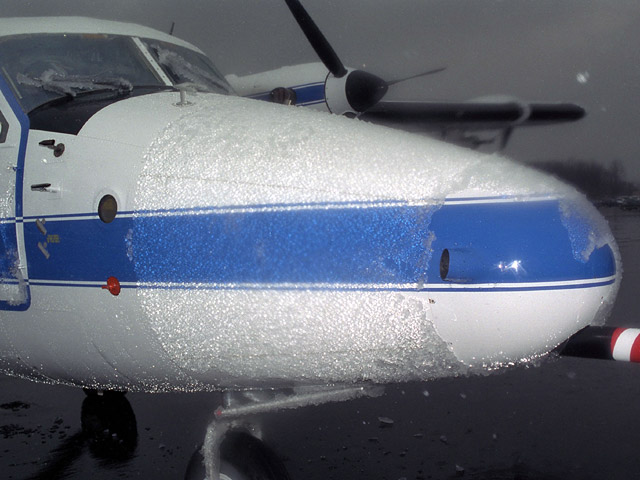
\includegraphics[scale=0.2]{Figures/Icing_on_a_plane.jpg}
        \hspace{0.1in}
        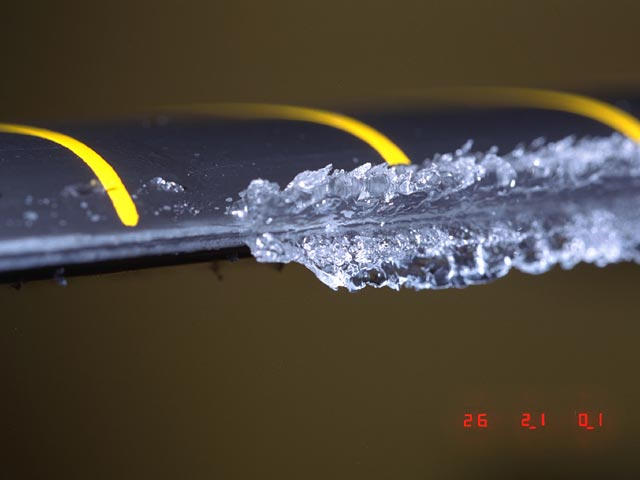
\includegraphics[scale=0.2]{Figures/Icing_on_a_rotor.jpg}
      \end{center}
      \begin{itemize}
        \item Industrial Coating
      \end{itemize}
    \end{frame}

    \begin{frame}
      \frametitle{Model Equations}
      \begin{itemize}
        \item Navier-Stokes Equation
          \begin{align*}
            \rho_t + \p{\rho u}_x &= 0 \\
            \p{\rho u}_t + \p{\rho u^2 + p}_x &=  \frac{4}{3Re} u_{xx} \\
            E_t + \p{u (E + p)}_x &= \frac{1}{Re} \p{\frac{2}{3} \p{u^2}_{xx} + \frac{\gamma}{(\gamma - 1)Pr} \p{\frac{p}{\rho}}_{xx}}
          \end{align*}
        \item Asymptotic Limit, $\rho << L$
        \item Thin-Film Equation - 1D with $q$ as fluid height.
          \[
            q_t + \p{f(x, t) q^2 - g(x, t) q^3}_x = -\p{h(x, t) q^3 q_{xxx}}_x
          \]
      \end{itemize}
    \end{frame}

    \begin{frame}
      \frametitle{Current Model}
      \begin{itemize}
        \item Simplified Expression
          \[
            q_t + \p{q^2 - q^3}_x = -\p{q^3 q_{xxx}}_x
          \]

        \item Operator Splitting
          \begin{align*}
            q_t + \p{q^2 - q^3}_x &= 0 \\
            q_t + \p{q^3 q_{xxx}}_x &= 0
          \end{align*}
      \end{itemize}
    \end{frame}

    \begin{frame}
      \frametitle{Introduction to Discontinuous Galerkin}
      \begin{itemize}
        \item Let $\mcT_h$ partition the domain, $\Omega = \br{a, b}$
          \[
            a = x_{1/2} < \cdots < x_{i-1/2} < x_{i+1/2} < \cdots < x_{N + 1/2} = b
          \]

        \item $K_i \in \mcT_h = \br{x_{i-1/2}, x_{i+1/2}}$
        \item $h = x_{i + 1/2} - x_{i - 1/2}$
        \item $x_i = \frac{x_{i+1/2} + x_{i-1/2}}{2}$.
          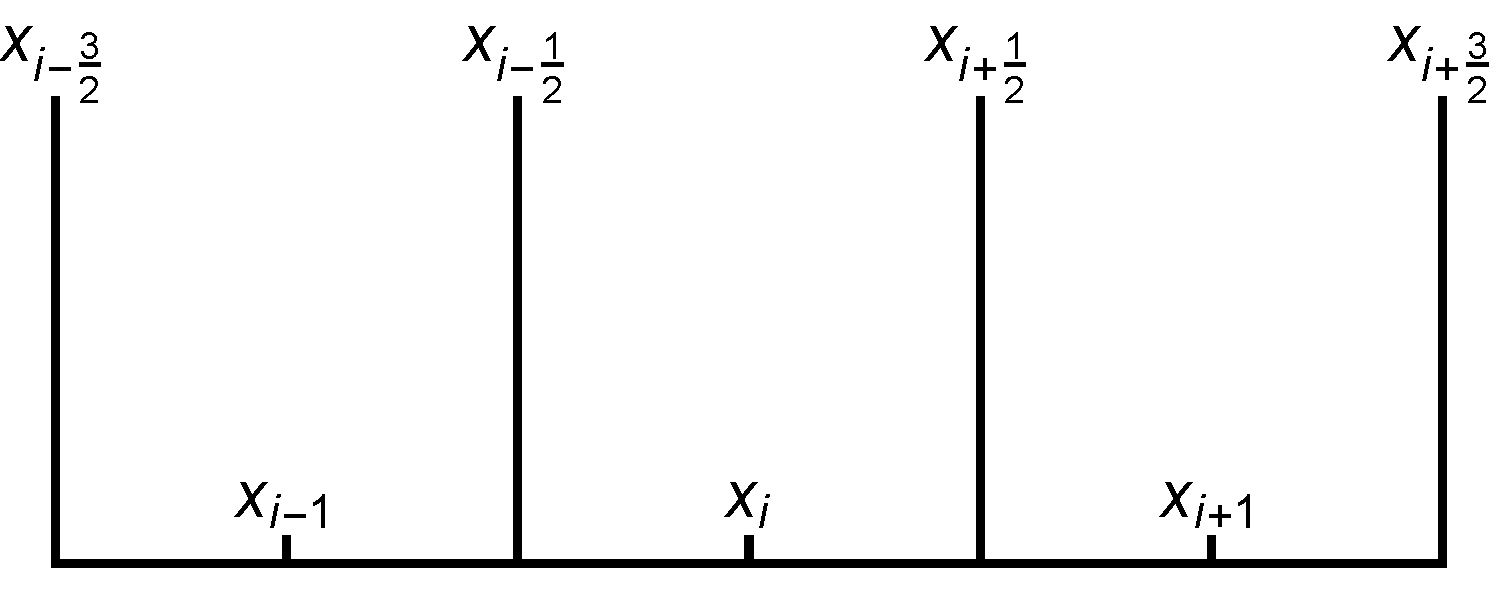
\includegraphics[scale=0.35]{Figures/Cells.pdf}
      \end{itemize}
    \end{frame}

    \begin{frame}
      \frametitle{Function Spaces}
      \begin{itemize}
        \item $P^k(K)$ - polynomials of degree less than or equal to $k$ on $K \in \mcT_h$
        \item 
          \[
            V_h = \set{v \in L^2(\Omega): \eval{v}{K} \in P^k(K), \quad \forall K \in \mcT_h}
          \]
      \end{itemize}
    \end{frame}

    \begin{frame}
      \frametitle{Numerical Solutions}
      \begin{itemize}
        \item Let $\set{\phi^k(\xi)}$ be the Legendre polynomials.

        \item Solution of order $M$ on each cell
          \[
            \eval{q}{x \in V_i}{} \approx Q_i = \sum*{k = 1}{M}{Q_i^k \phi^k(\xi)}
          \]
          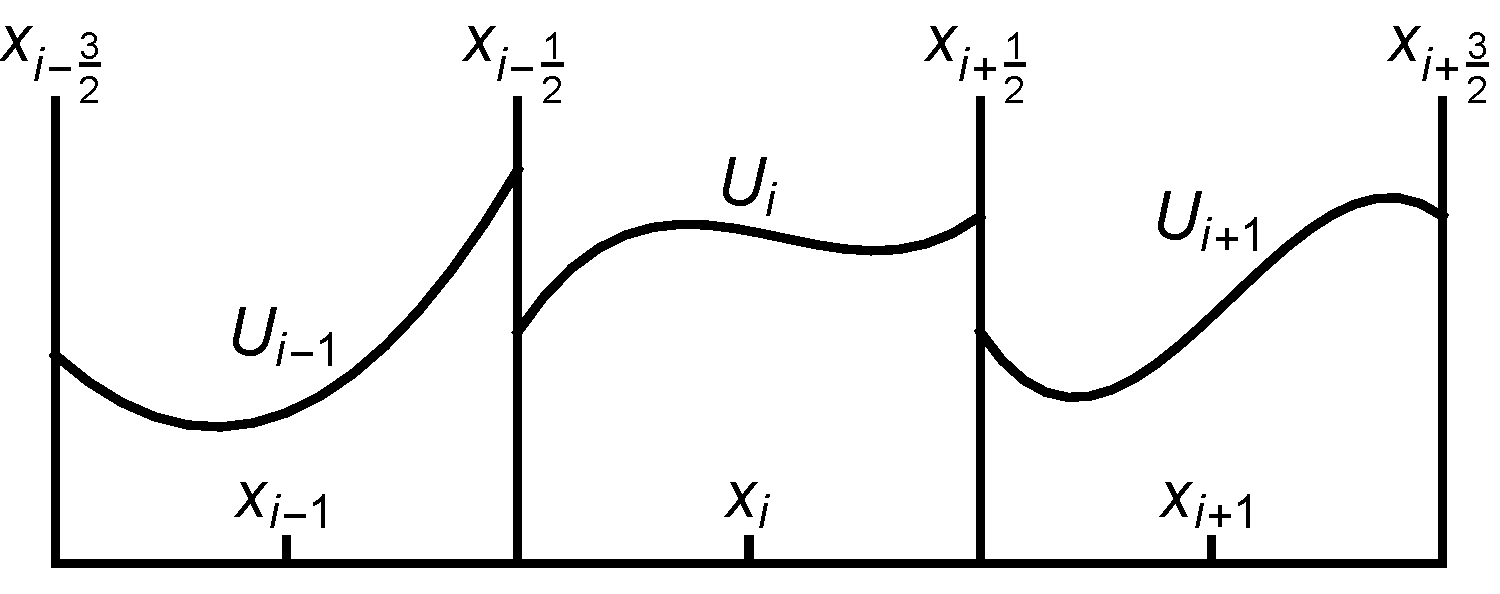
\includegraphics[scale=0.35]{Figures/DG.pdf}
      \end{itemize}
    \end{frame}

  \section{Convection}
    \begin{frame}
      \frametitle{Convection}
      \begin{itemize}
        \item Convection Equation
          \begin{gather*}
            q_t + \frac{2}{\Delta x} f(q)_\xi = 0 \\
            f(q) = q^2 - q^3
          \end{gather*}

        \item Weak Form
          \[
            \dintt*{-1}{1}{q_t \phi(\xi) + \frac{2}{\Delta x}f(q)_\xi \phi(\xi)}{\xi} = 0
          \]

        \item Runge-Kutta Discontinuous Galerkin
          \[
            \dot{Q_i^{\ell}} = \frac{1}{\Delta x}\dintt{-1}{1}{f(Q_i)\phi_{\xi}^{\ell}}{\xi} - \frac{1}{\Delta x} \p{\mcF_{i + 1/2} - \mcF_{i - 1/2}}
          \]

        \item Rusanov Numerical Flux
          \[
            \mcF_{j+1/2} = \frac{f\p{Q_{i+1}(-1)} + f\p{Q_{i}(1)}}{2} \phi^{\ell}(1)
          \]

        \item Solve this system of ODEs with any Explicit Strong Stability Preserving (SSP) Runge-Kutta Method.
      \end{itemize}
    \end{frame}

    \begin{frame}
      \frametitle{Numerical Example - Square Wave}
      \begin{center}
        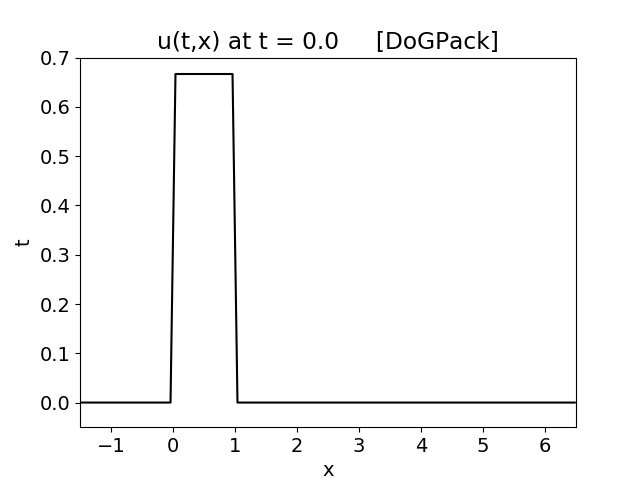
\includegraphics[scale=0.6]{Figures/squarewave00.png}
      \end{center}
    \end{frame}
    \begin{frame}
      \frametitle{Numerical Example - Square Wave}
      \begin{center}
        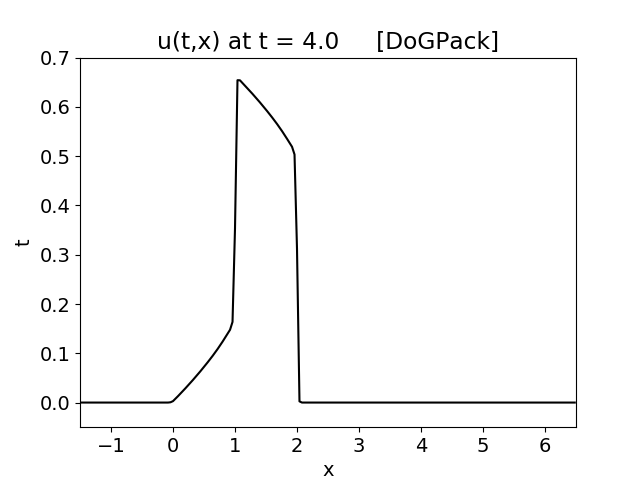
\includegraphics[scale=0.6]{Figures/squarewave04.png}
      \end{center}
    \end{frame}
    \begin{frame}
      \frametitle{Numerical Example - Square Wave}
      \begin{center}
        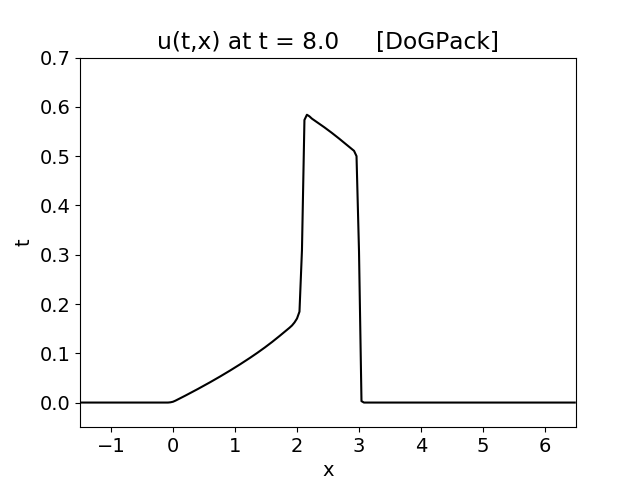
\includegraphics[scale=0.6]{Figures/squarewave08.png}
      \end{center}
    \end{frame}
    \begin{frame}
      \frametitle{Numerical Example - Square Wave}
      \begin{center}
        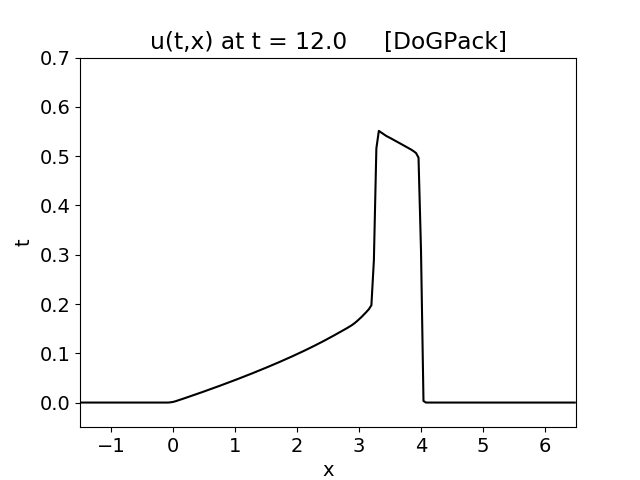
\includegraphics[scale=0.6]{Figures/squarewave12.png}
      \end{center}
    \end{frame}
    \begin{frame}
      \frametitle{Numerical Example - Square Wave}
      \begin{center}
        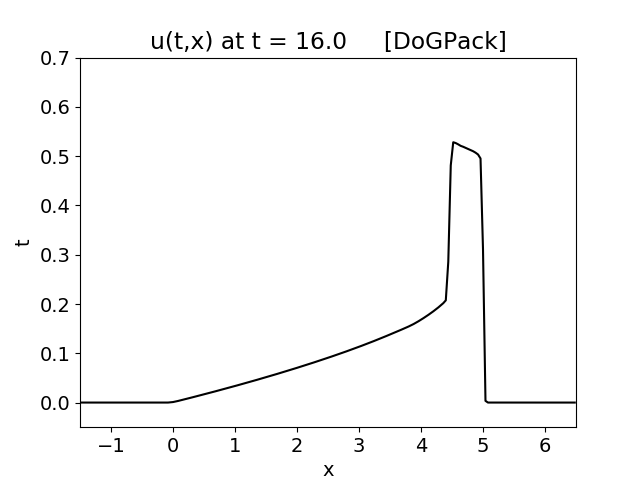
\includegraphics[scale=0.6]{Figures/squarewave16.png}
      \end{center}
    \end{frame}
    \begin{frame}
      \frametitle{Numerical Example - Square Wave}
      \begin{center}
        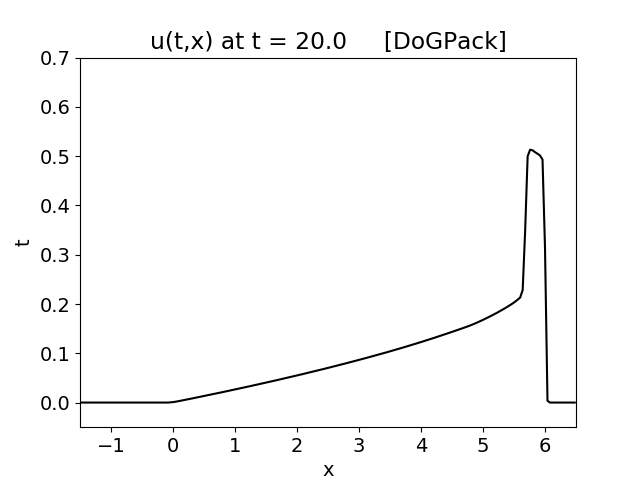
\includegraphics[scale=0.6]{Figures/squarewave20.png}
      \end{center}
    \end{frame}

  \section{Hyper-Diffusion}
    \begin{frame}
      \frametitle{Hyper-Diffusion}
      \begin{itemize}
        \item Hyper-Diffusion Equation
          \[
            u_t + \frac{16}{\Delta x^4} \p{u^3 u_{\xi\xi\xi}}_\xi = 0
          \]

        \item Local Discontinuous Galerkin (LDG)
          \begin{align*}
            q &= \frac{2}{\Delta x} u_{\xi} \\
            r &= \frac{2}{\Delta x} q_{\xi} \\
            s &= \frac{2}{\Delta x} u^3 r_{\xi} \\
            u_t &= -\frac{2}{\Delta x} s_{\xi}
          \end{align*}
      \end{itemize}
    \end{frame}

    \begin{frame}
      \frametitle{Local Discontinuous Galerkin}
      \begin{align*}
        \eta(\xi) &= \p{U_i^{n}}^3 \\
        Q_i^{\ell} &= -\frac{1}{\Delta x} \p{\dintt{-1}{1}{U_i \phi_{\xi}^{\ell}}{\xi}
        - \mcF(U)_{i+1/2}^{\ell} + \mcF(U)_{i - 1/2}^{\ell}} \\
        R_i^{\ell} &= -\frac{1}{\Delta x} \p{\dintt{-1}{1}{Q_i \phi_{\xi}^{\ell}}{\xi}
        - \mcF(Q)_{i+1/2}^{\ell} + \mcF(Q)_{i - 1/2}^{\ell}} \\
        S_i^{\ell} &= \frac{1}{\Delta x} \p{\dintt{-1}{1}{(R_i)_{\xi} \eta(\xi) \phi^{\ell}}{\xi}} \\
        &+ \frac{1}{\Delta x}\p{\mcF(\eta)_{i + 1/2} \mcF(R)_{i+1/2}^{\ell} - \mcF(\eta)_{i-1/2} \mcF(R)_{i-1/2}^{\ell}}\\
        \dot{U}_i^{\ell} &= \frac{1}{\Delta x} \p{\dintt{-1}{1}{S_i \phi_{\xi}^{\ell}}{\xi}
        - \mcF(S)_{i+1/2}^{\ell} + \mcF(S)_{i - 1/2}^{\ell}}
      \end{align*}
    \end{frame}

    \begin{frame}
      \frametitle{Local Discontinuous Galerkin}
      \begin{align*}
        \mcF(\eta)_{i+1/2} &= \frac{1}{2}\p{\eta_{i+1}(-1) - \eta_{i}(1)} \\
        \mcF(\eta)_{i-1/2} &= \frac{1}{2}\p{\eta_{i-1}(1) - \eta_{i}(-1)} \\
        \mcF(*)_{i+1/2}^{\ell} &= \phi^{\ell}(1) *_{i+1/2}
      \end{align*}
      \begin{center}
        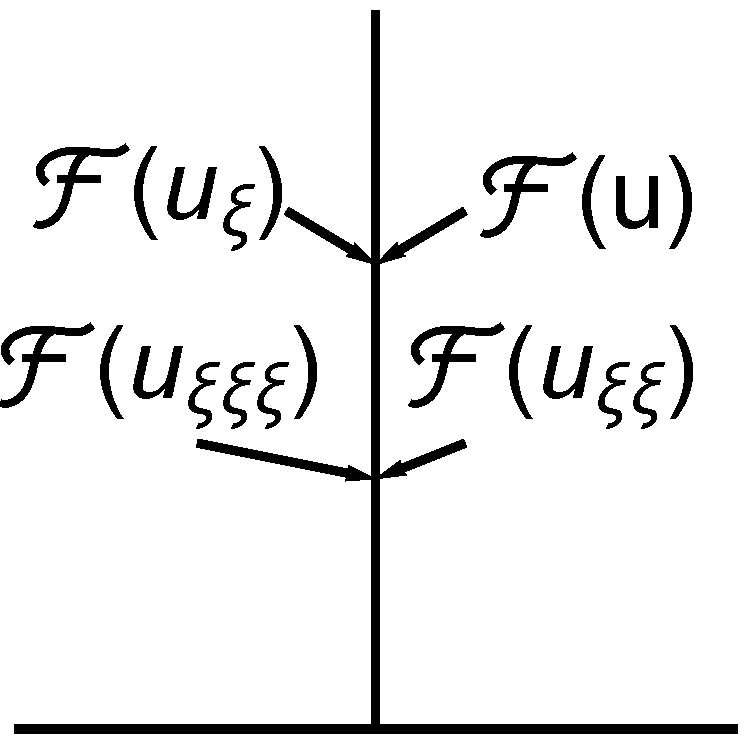
\includegraphics[scale=0.3]{Figures/localDG.pdf}
      \end{center}
    \end{frame}

    \begin{frame}
      \frametitle{Local Discontinuous Galerkin}
      \begin{itemize}
        \item Explicit SSP Runge Kutta
          \begin{itemize}
            \item Severe time step restriction
            \item $\Delta t \sim \Delta x^4$
            \item $\Delta x = .1 \to \Delta t \approx 10^{-4}$
            \item $\Delta x = .01 \to \Delta t \approx 10^{-8}$
          \end{itemize}

        \item Implicit SSP Runge Kutta
          \begin{itemize}
            \item Linear System Solver
            \item Stabilized BiConjugate Gradient
            \item MultiGrid Solver
          \end{itemize}
      \end{itemize}
    \end{frame}

  \section{Operator Splitting}
    \begin{frame}
      \frametitle{Operator Splitting}
      \begin{itemize}
        \item Strang Splitting
          \begin{itemize}
            \item 1 time step
              \begin{itemize}
                \item 1/2 time step for convection
                \item 1 time step for hyper-diffusion
                \item 1/2 time step for convection
              \end{itemize}
            \item Second order splitting
          \end{itemize}
      \end{itemize}
    \end{frame}

    \begin{frame}
      \frametitle{Numerical Results - Riemann Problem}
      \begin{center}
        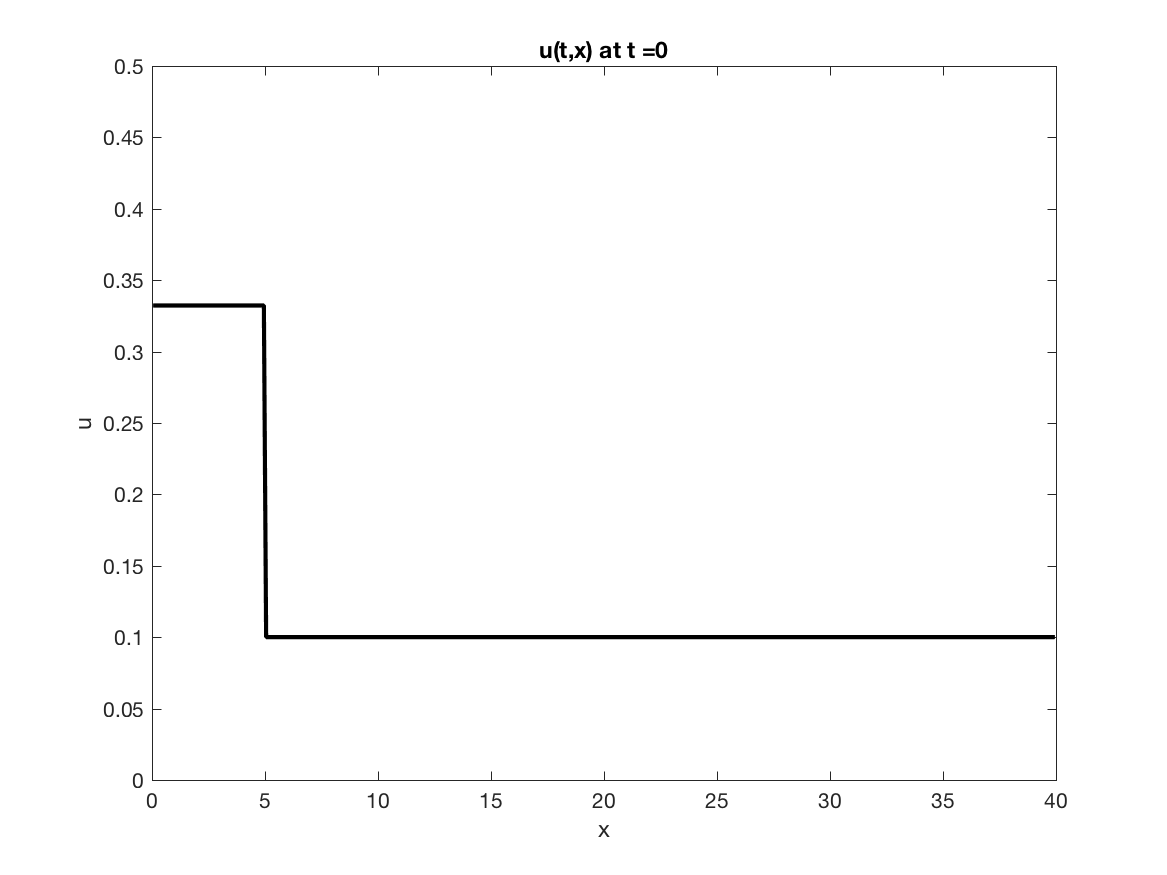
\includegraphics[scale=0.5]{Figures/reimann0.png}
      \end{center}
    \end{frame}
    \begin{frame}
      \frametitle{Numerical Results - Riemann Problem}
      \begin{center}
        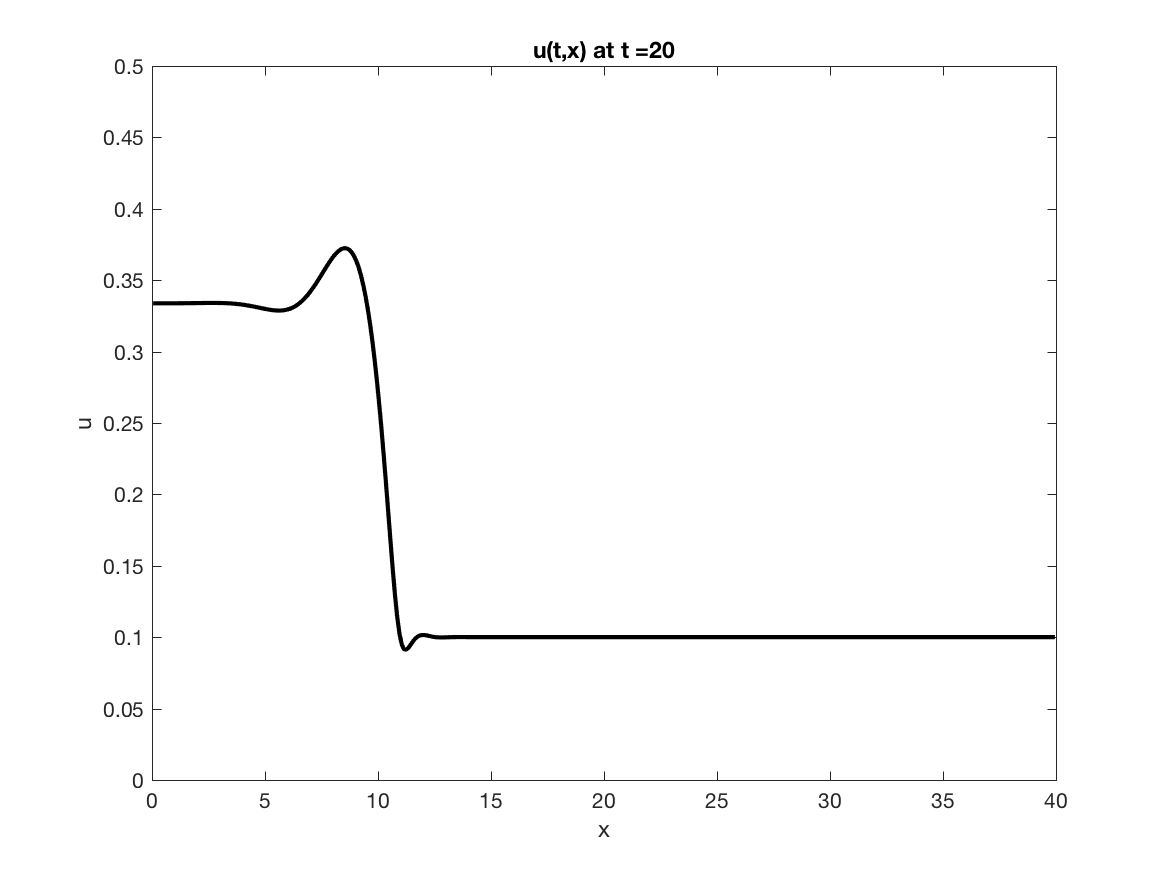
\includegraphics[scale=0.5]{Figures/reimann20.png}
      \end{center}
    \end{frame}
    \begin{frame}
      \frametitle{Numerical Results - Riemann Problem}
      \begin{center}
        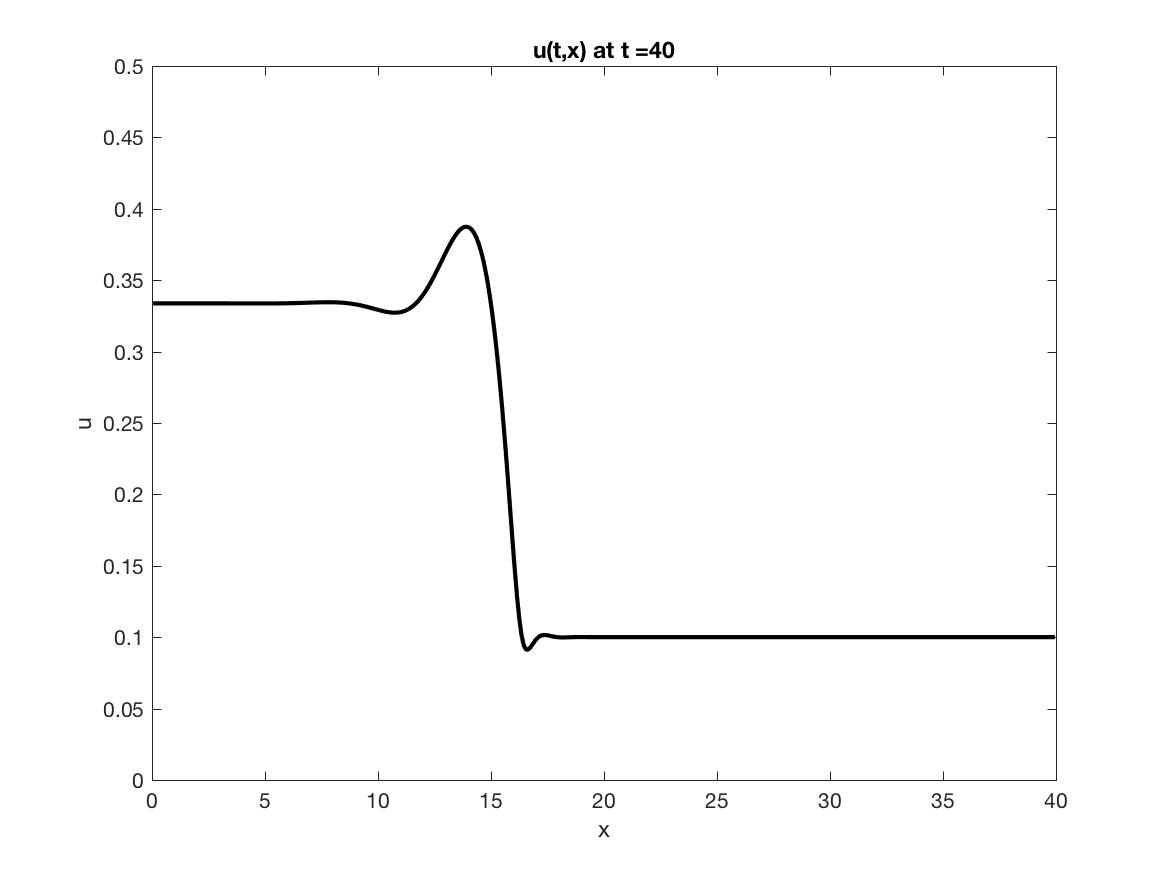
\includegraphics[scale=0.5]{Figures/reimann40.png}
      \end{center}
    \end{frame}
    \begin{frame}
      \frametitle{Numerical Results - Riemann Problem}
      \begin{center}
        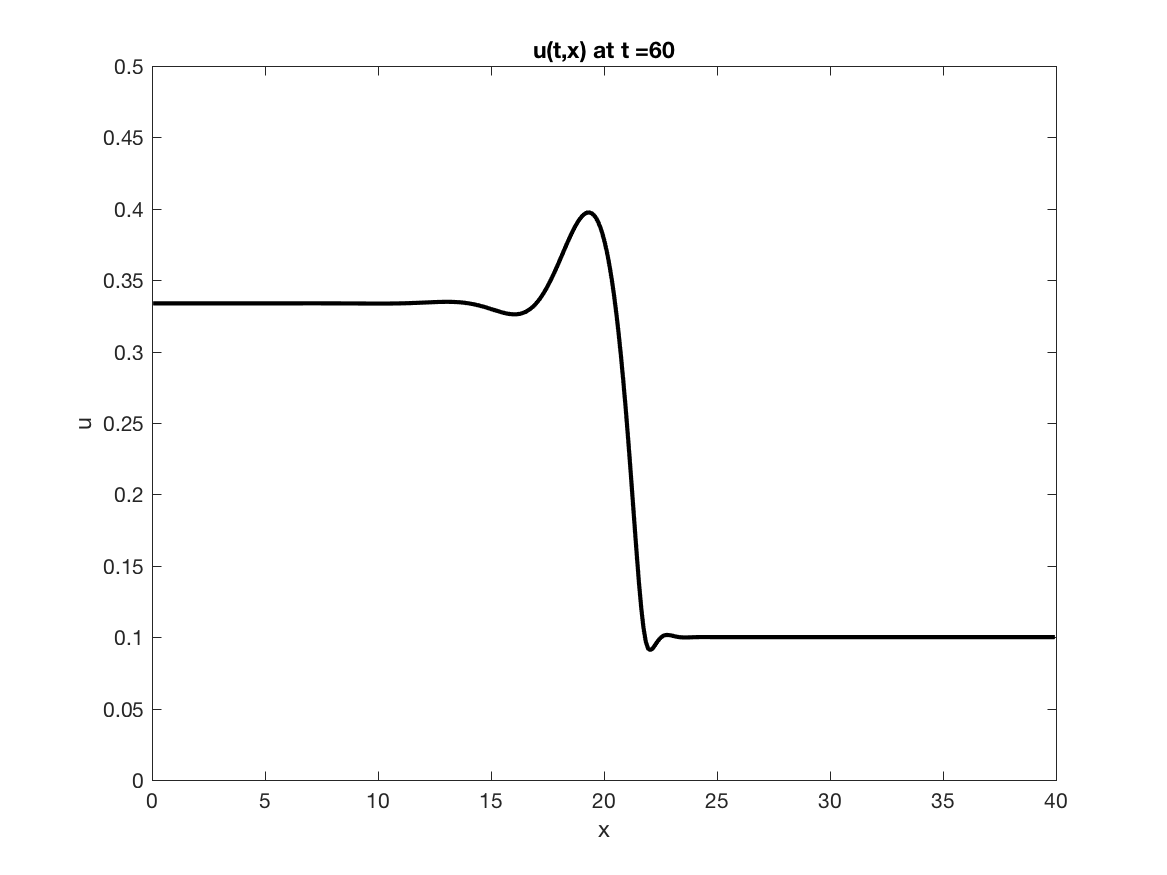
\includegraphics[scale=0.5]{Figures/reimann60.png}
      \end{center}
    \end{frame}
    \begin{frame}
      \frametitle{Numerical Results - Riemann Problem}
      \begin{center}
        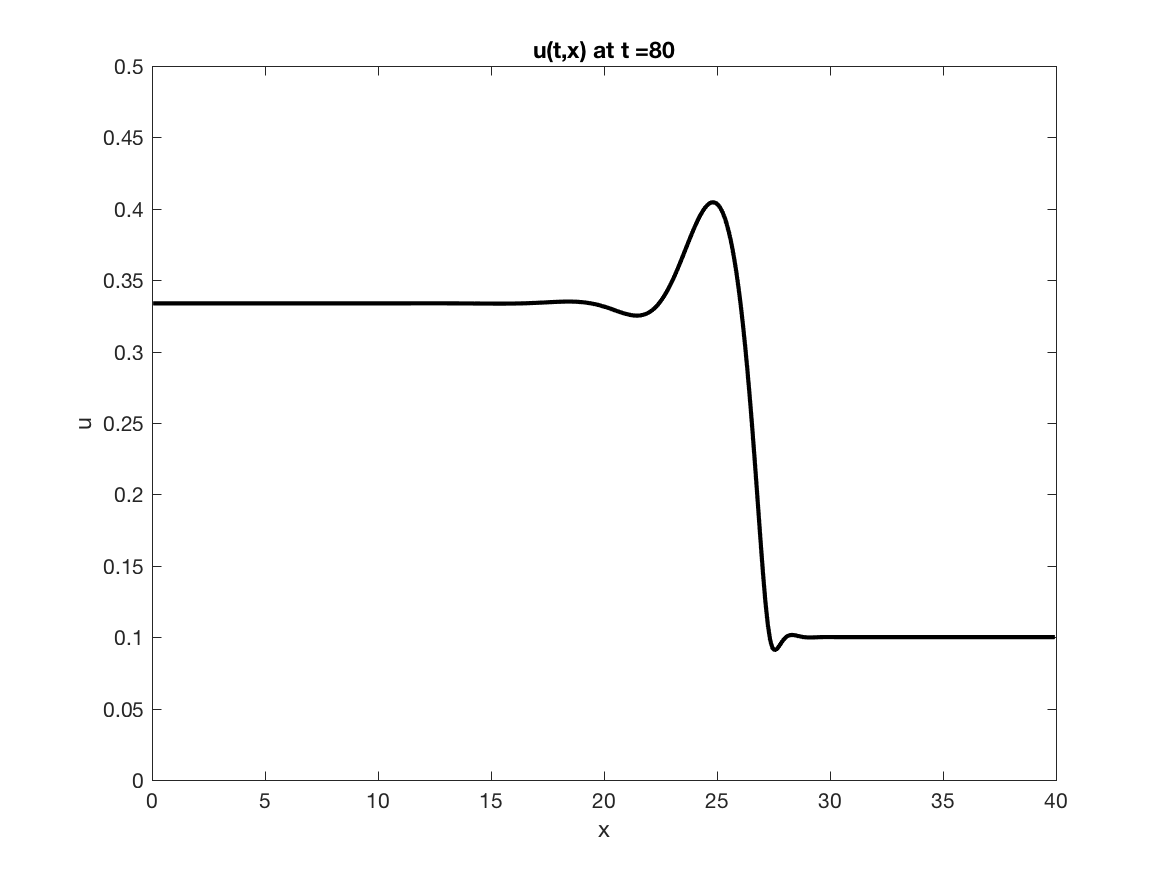
\includegraphics[scale=0.5]{Figures/reimann80.png}
      \end{center}
    \end{frame}
    \begin{frame}
      \frametitle{Numerical Results - Riemann Problem}
      \begin{center}
        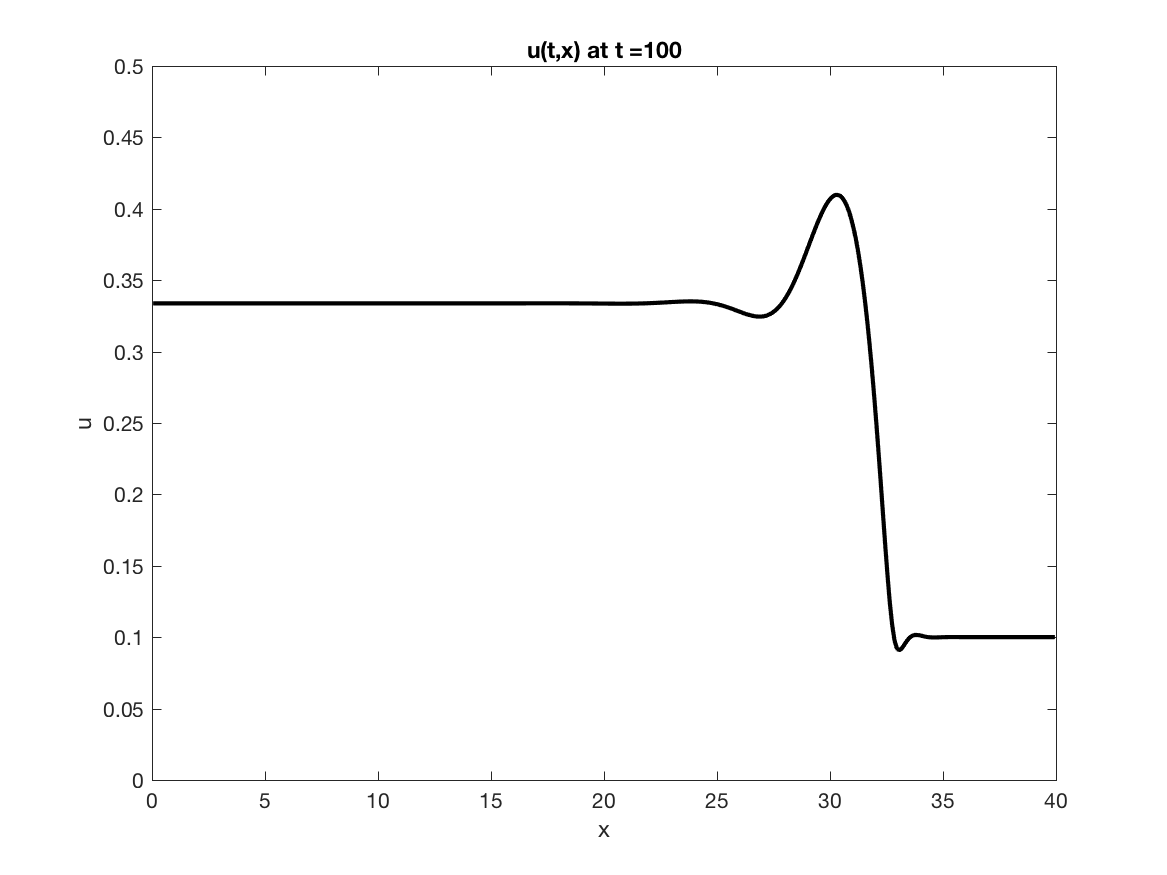
\includegraphics[scale=0.5]{Figures/reimann100.png}
      \end{center}
    \end{frame}

  \section{Conclusion}
    \begin{frame}
      \frametitle{Future Work}
      \begin{itemize}
        \item Higher dimensions
        \item Curved surfaces
        \item Space and time dependent coefficients
        \item Incorporation with air flow models
        \item Runge Kutta IMEX
      \end{itemize}
    \end{frame}

    \begin{frame}
      \frametitle{Conclusion}
      \begin{itemize}
        \item Thanks
          \begin{itemize}
            \item James Rossmanith
            \item Alric Rothmayer
          \end{itemize}
        \item Questions?
      \end{itemize}
    \end{frame}

    \begin{frame}
      \frametitle{Bibliography}
      % TODO: Bibliography
      \nocite{*}
      \printbibliography{}
    \end{frame}
\end{document}
